\section{City Selection}
\label{sec:city-selection}

This section presents an explanation of the city selection process.

\subsection{Criteria}

We carefully selected among several candidate cities, using the following criteria:

\begin{itemize}
    \item A city the team is familiar with, so that we can better understand the practical implications of our work.
    \item A city with well-defined borders, so that we can easily define a realistic environment.
    \item A city with reasonable complexity, not too big and not too small.
\end{itemize}

\subsection{Candidate Cities}

We selected the following cities for consideration:
\begin{enumerate}
    \item \textbf{Barcelona, Spain:} Our city, but relatively dense and complex.
    \item \textbf{Seville, Spain:} Similarly very dense and complex.
    \item \textbf{Salamanca, Spain:} Not as dense or complex, but lacks well-defined borders.
    \item \textbf{Tossa de Mar, Spain:} Small and very compact. Includes a long single road.
    \item \textbf{Lloret de Mar, Spain:} Relatively small, but includes densely connected city areas.
    \item \textbf{New York, NY, USA:} Prohibitively large and complex.
\end{enumerate}

\subsection{Evaluation}

\begin{figure}[htbp]
    \centering
    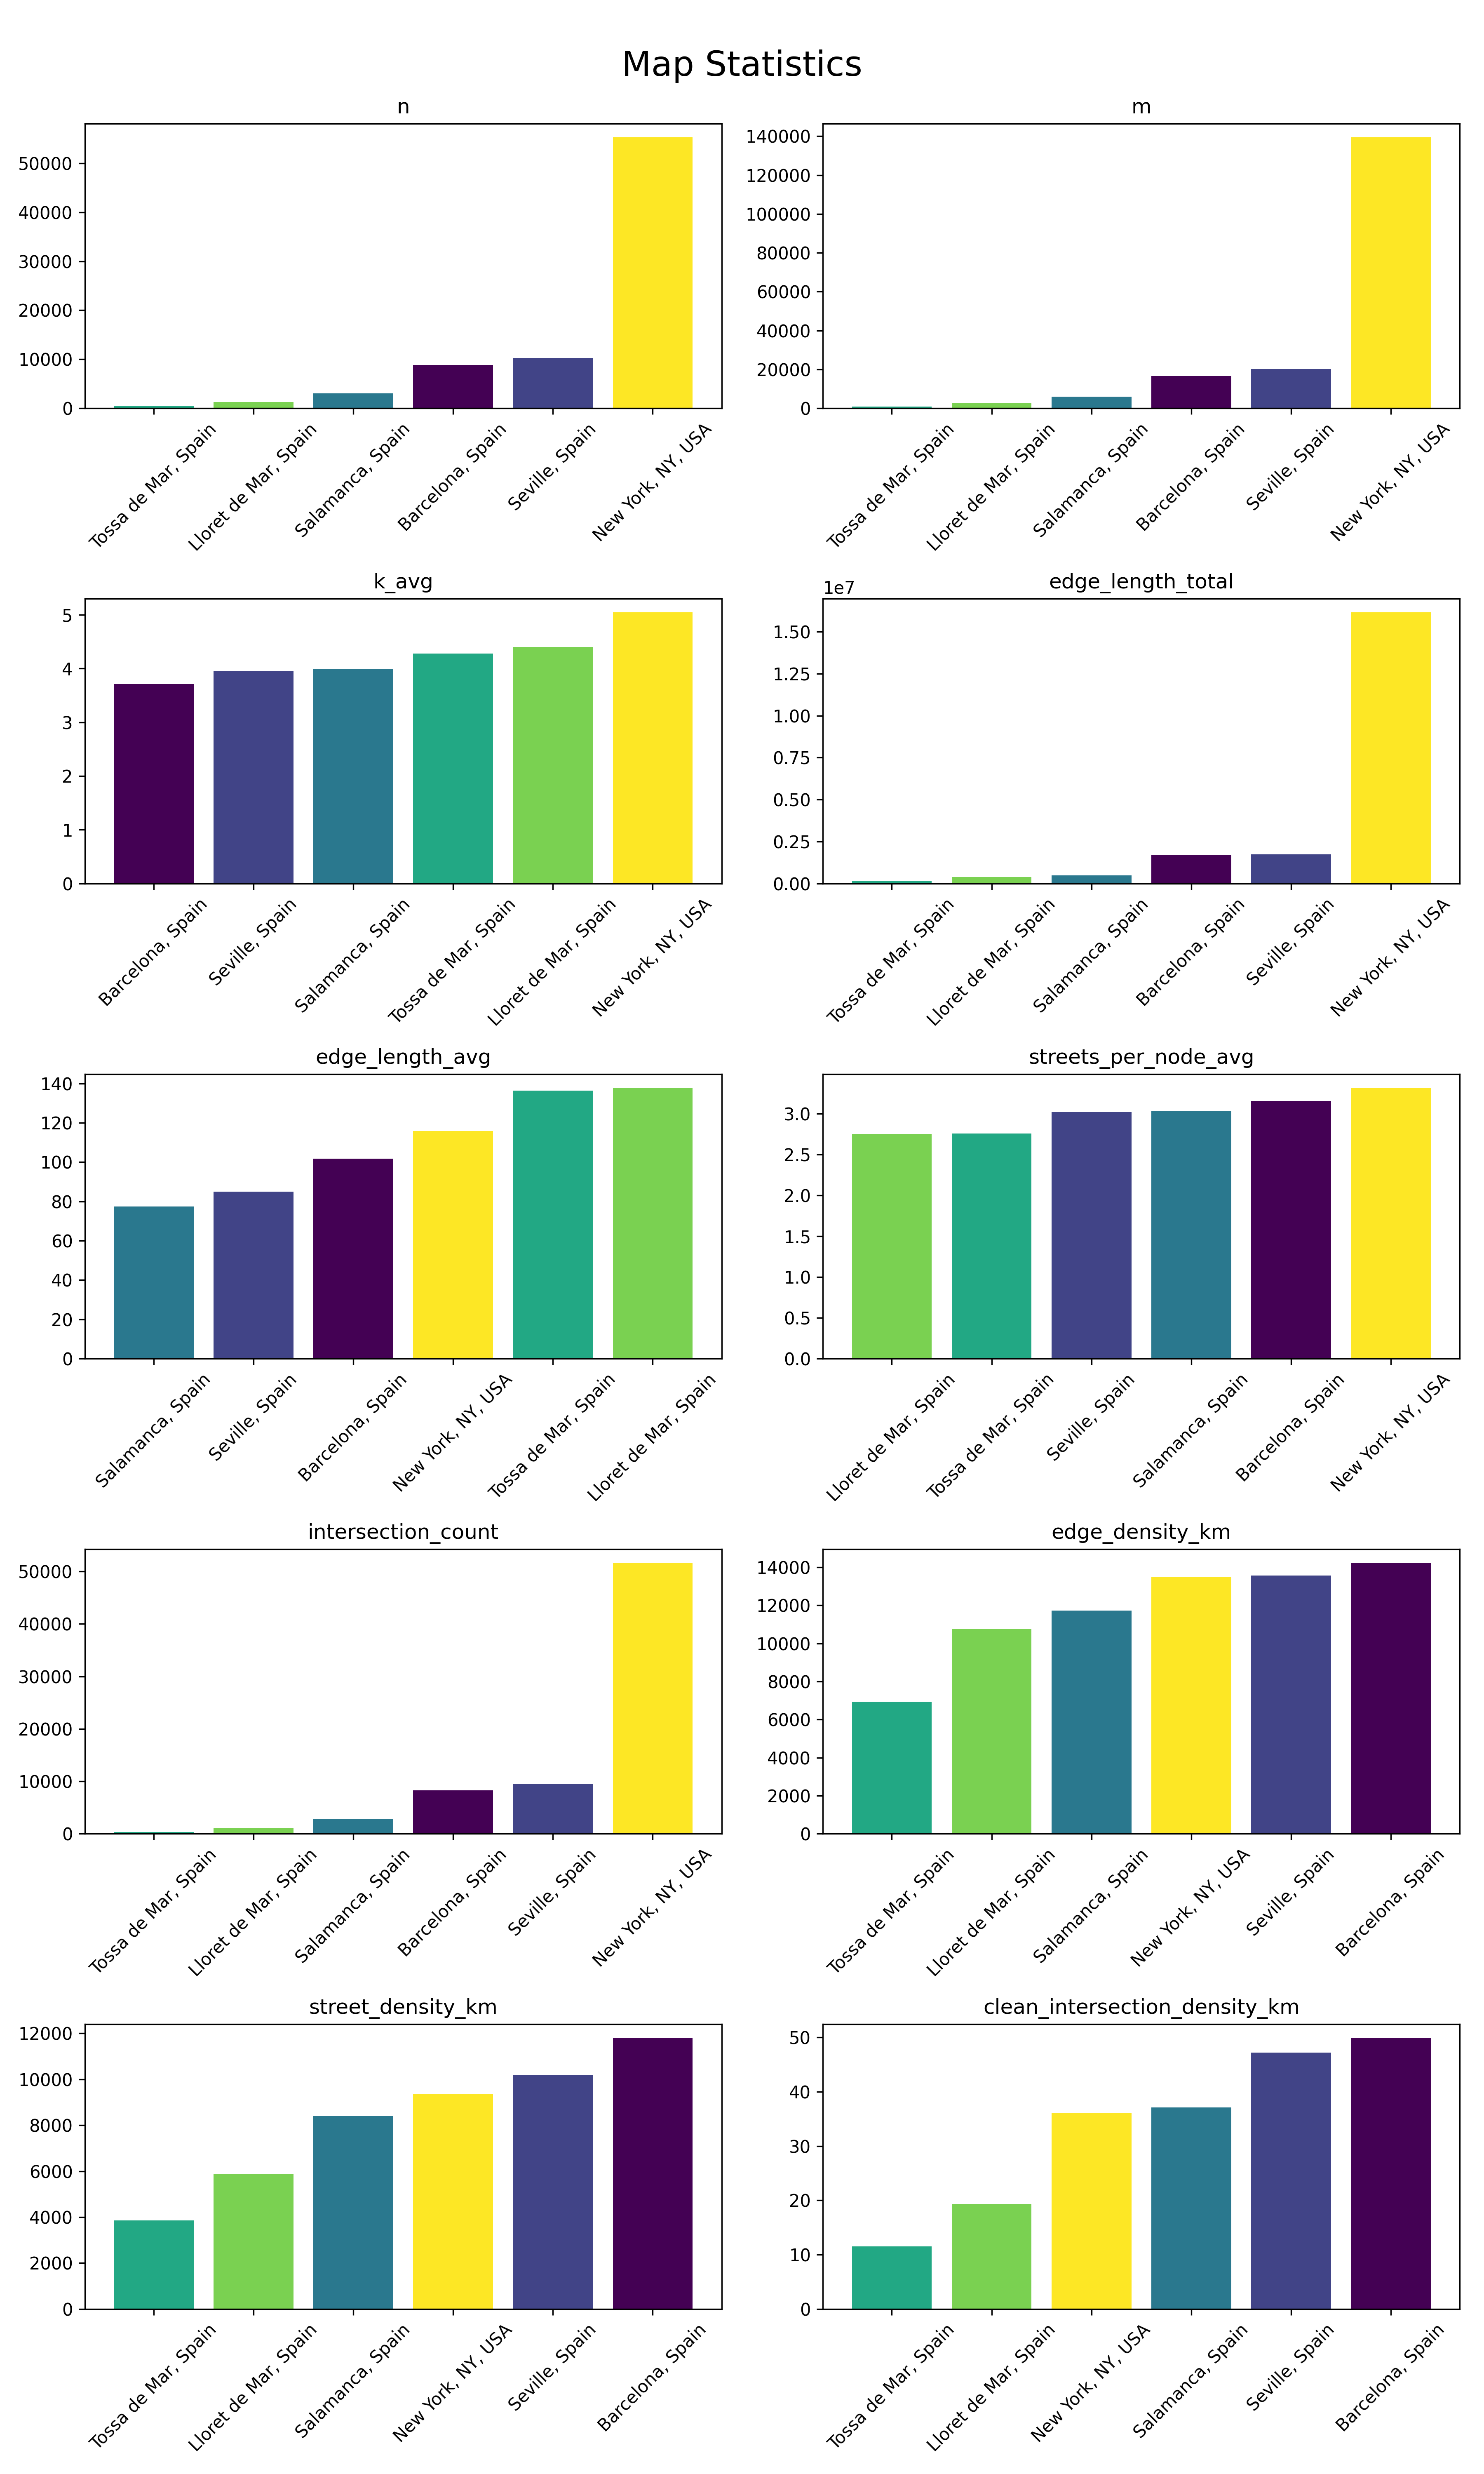
\includegraphics[width=0.8\textwidth]{../figures/map_complexity_statistics.png}
    \caption{Map Complexity Statistics}
    \label{fig:map-complexity-statistics}
\end{figure}

We pulled 10 metrics from the OSMnx package\cite{boeing2024osmnx} for each city. Plots of
these metrics are shown in \autoref{fig:map-complexity-statistics}.
\begin{itemize}
    \item \texttt{n}: Number of nodes in the graph
    \item \texttt{m}: Number of edges in the graph  
    \item \texttt{k\_avg}: Average node degree
    \item \texttt{edge\_length\_total}: Total length of all edges in meters
    \item \texttt{edge\_length\_avg}: Average edge length in meters
    \item \texttt{streets\_per\_node\_avg}: Average number of streets per node
    \item \texttt{intersection\_count}: Number of intersections
    \item \texttt{edge\_density\_km}: Kilometers of edge per square kilometer
    \item \texttt{street\_density\_km}: Kilometers of street per square kilometer
    \item \texttt{clean\_intersection\_count}: Number of intersections (cleaned)
\end{itemize}

\begin{figure}[htbp]
    \centering
    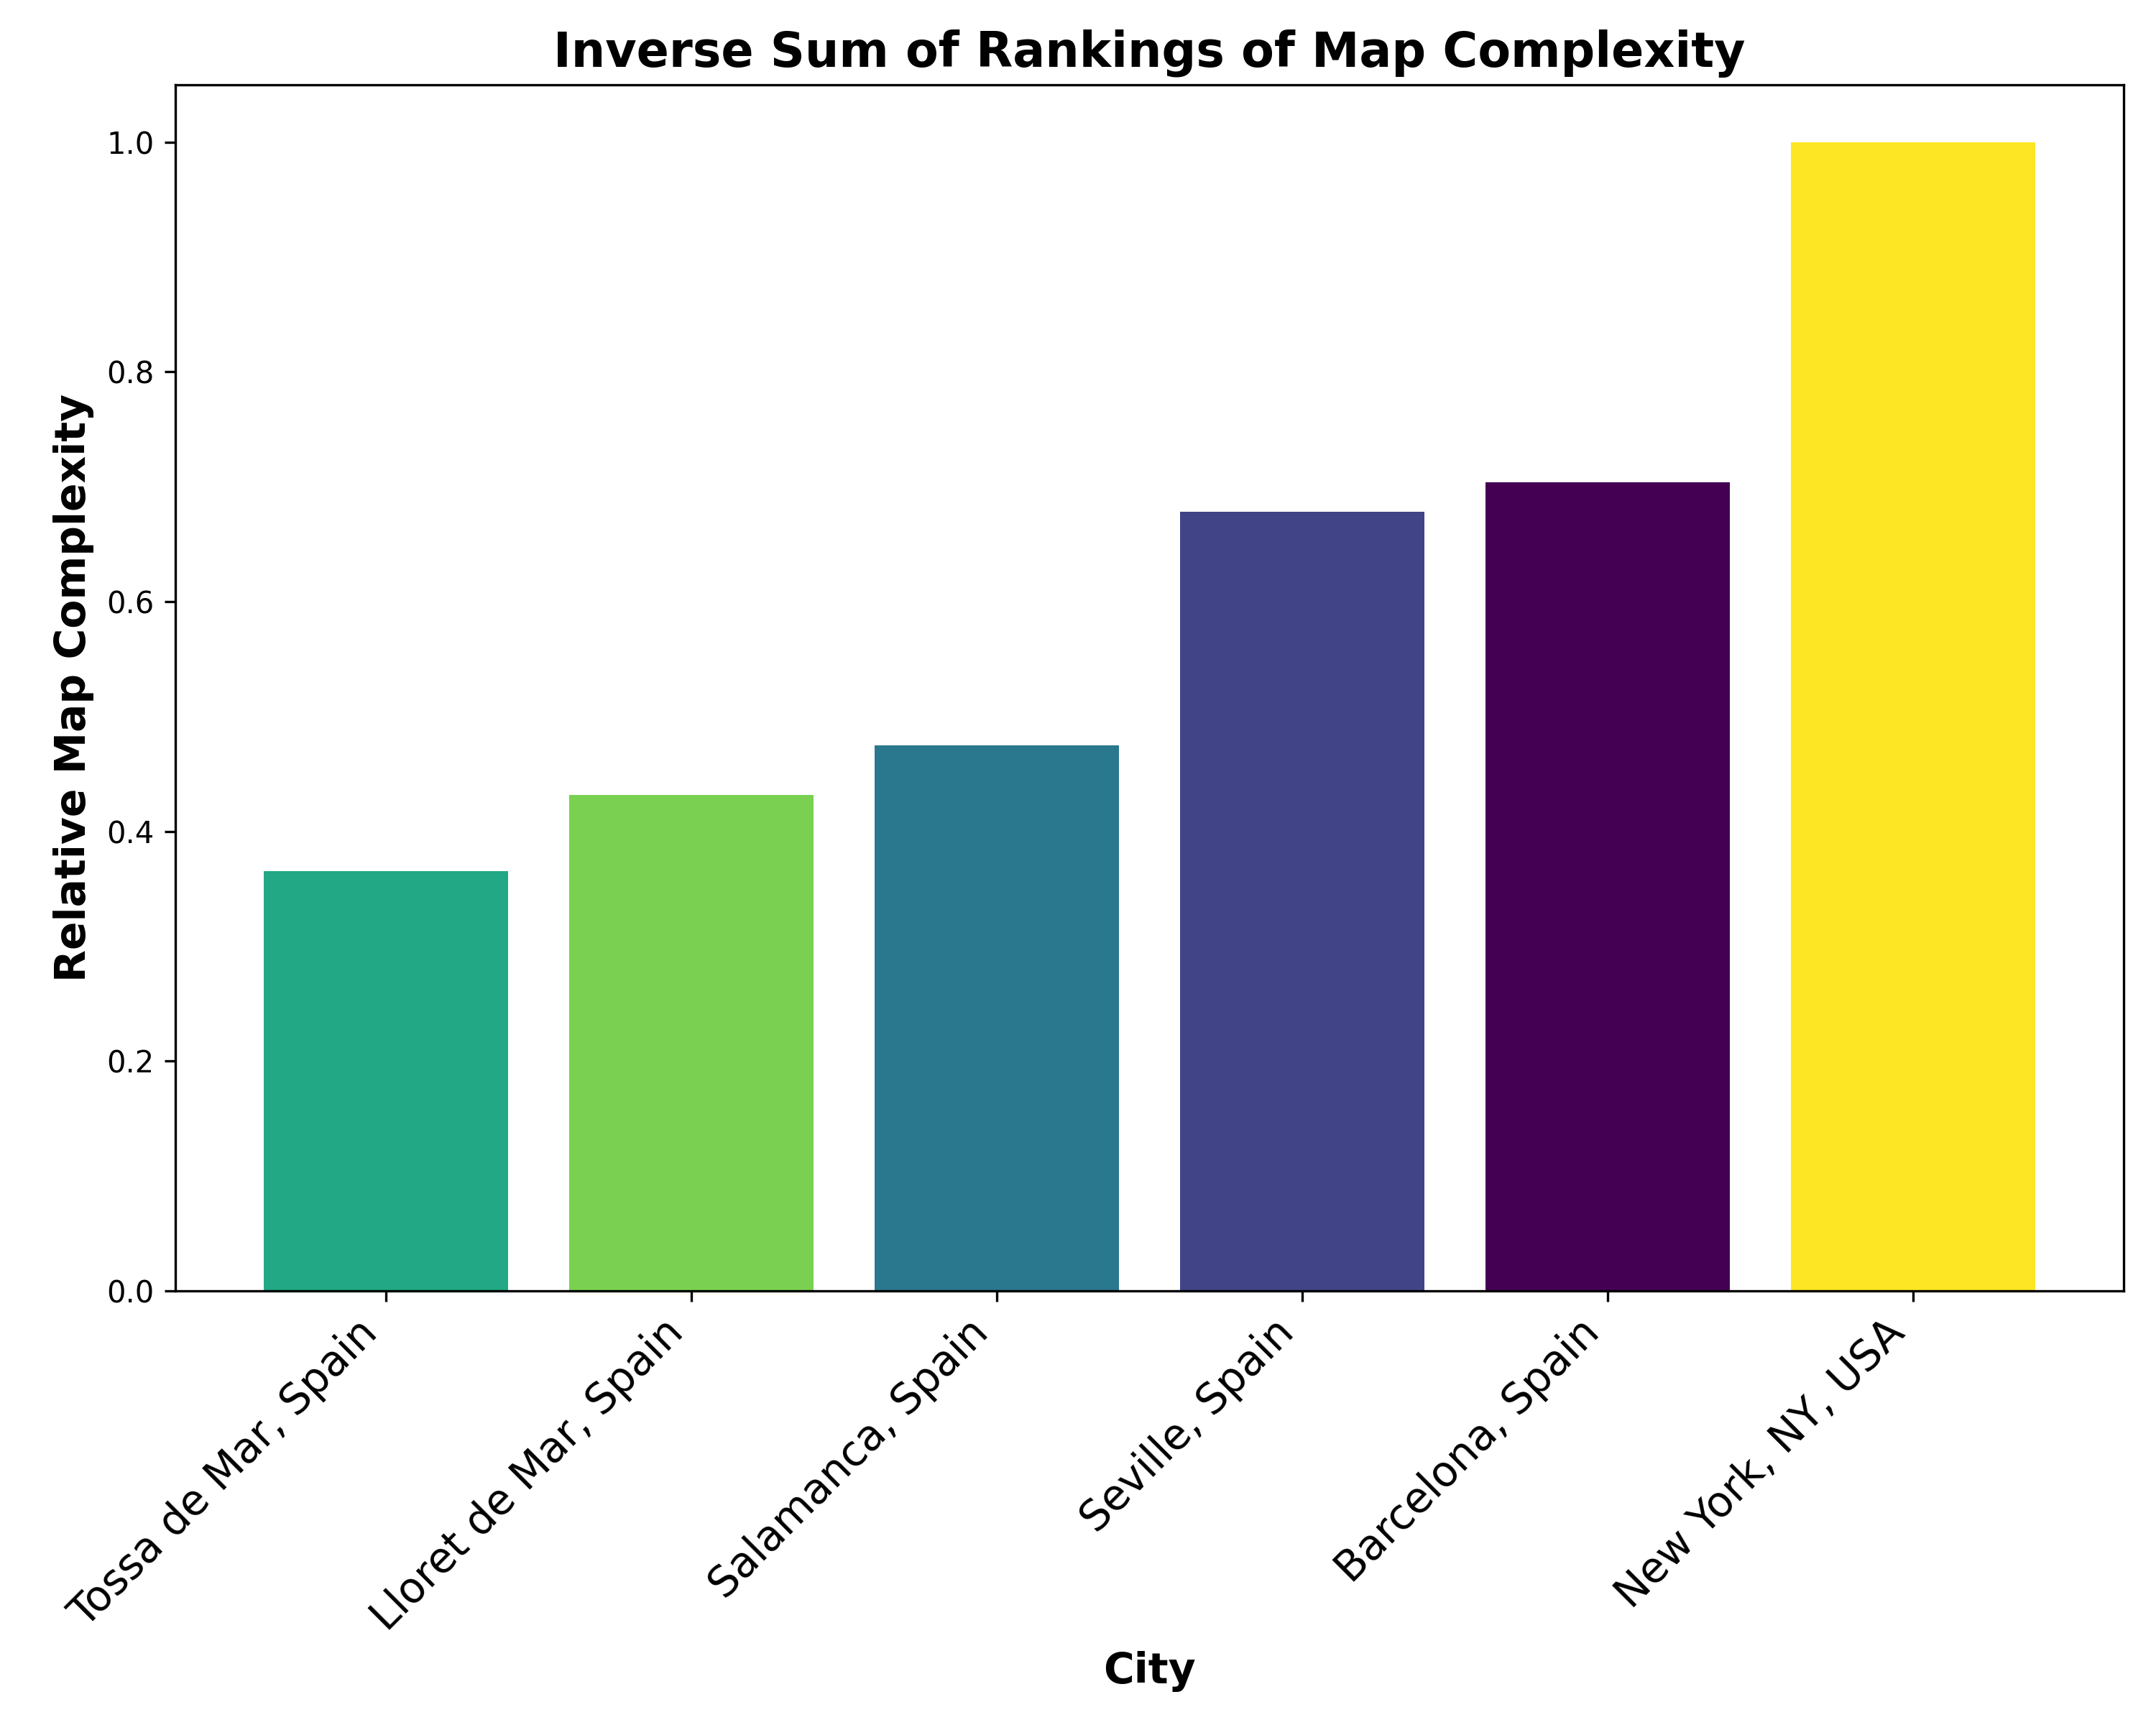
\includegraphics[width=0.4\textwidth]{../figures/relative_map_complexity.png}
    \caption{Relative Map Complexity}
    \label{fig:relative-map-complexity}
\end{figure}

We ranked each city based on each metric, and then added the ranks, inverted them,
and normalized them to derive a relative complexity score.
As you can see in \autoref{fig:relative-map-complexity},
\textbf{New York} is by far the most complex city, and \textbf{Tossa de Mar} is the least complex.
\textbf{Barcelona}, \textbf{Seville}, and \textbf{Salamanca} are of similar moderate complexity.

\subsection{Selection: Lloret de Mar}

We decided to select \textbf{Lloret de Mar} because it has a more interesting structure
than the other large Spanish cities, but has a more standard layout and
complexity than \textbf{Tossa de Mar}. This makes it a nice, well-balanced case study (see \autoref{fig:candidate-cities}).

\begin{figure}[H]
    \centering
    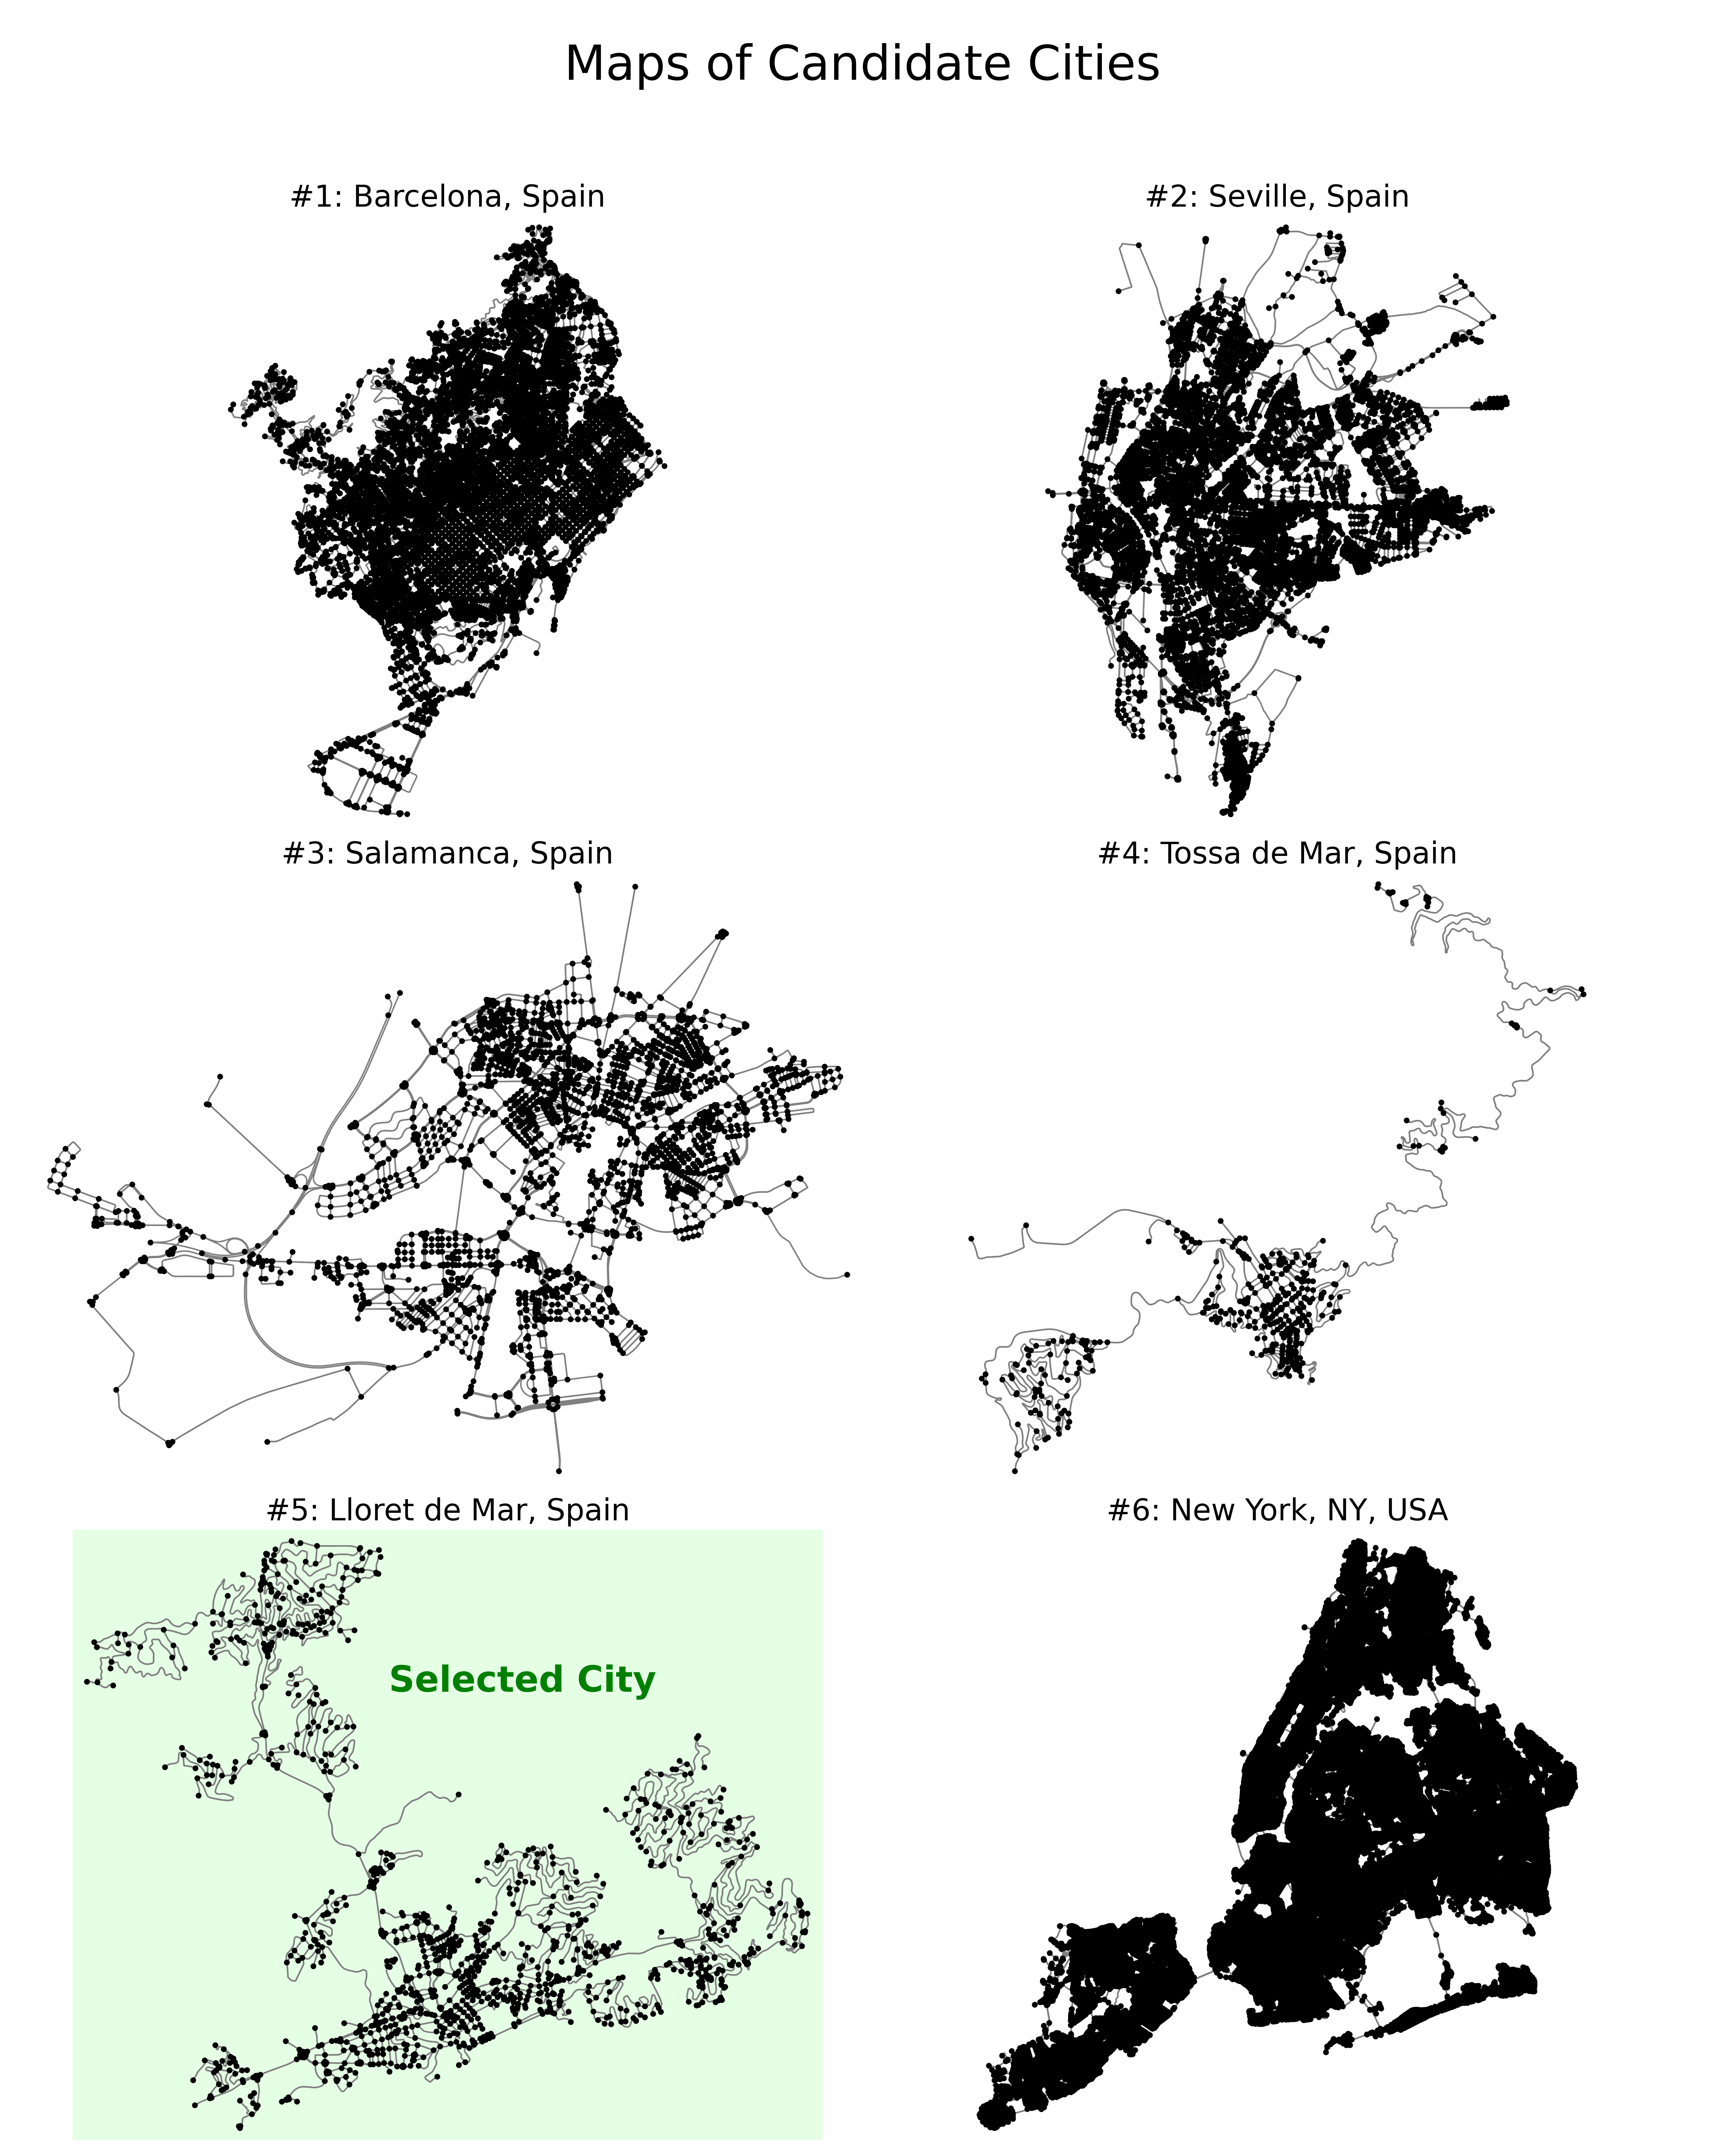
\includegraphics[width=\textwidth]{../figures/maps_of_candidate_cities.png}
    \caption{Maps of Candidate Cities}
    \label{fig:candidate-cities}
\end{figure}